\section{Sequential Decision Making}
RL is stochastic control process in discrete time \cite{sutton_reinforcement_1998}. At time $t$, the agent starts with state $s_t$ and observes $o_t$, then takes action $a_t$ according to its policy $\pi$ and obtains reward $r_t$ at time $t$. Then state transition to $s_{t+1}$ as a consequence of action and agent observes next observation $o_{t+1}$. History is set of past actions observations and rewards, $h_t=\{ a_0, o_0, r_0, ... a_t, o_t, r_t\}$. State $s_t$ is function of the history, $s_t=f(h_t)$, which represents situtaion of environment as much as possible. The RL diagram is visualized in \figref{fig:rl_diagram}. \\
\begin{figure}
	\centering
	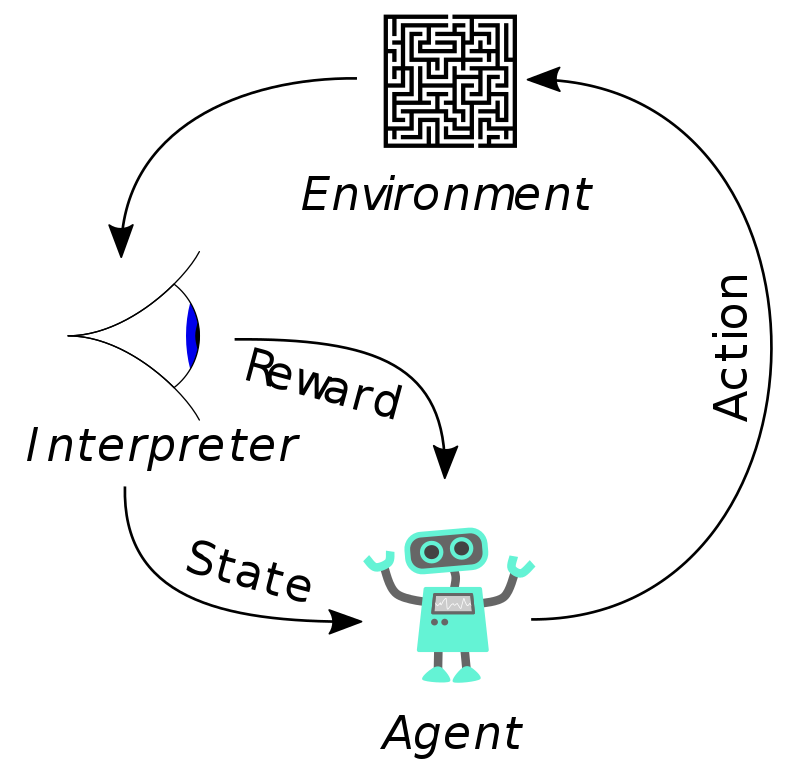
\includegraphics[width=0.7\textwidth]{figures/ml_theory/RL_diagram.png}
	\caption{Reinforcement Learning Diagram}
	\label{fig:rl_diagram}
\end{figure}

\section{Markov Decision Process}
\label{sec:mdp}
Markov Decision Process (MDP) is a sequential decision making process with Markov property. It is represented as a tuple $(\mathcal{S},\mathcal{A},T,R,\gamma)$. Markov property means that the conditional probability distribution of the future state depends only on the instant state and action instead of the entire past, so it is memoryless. In MDP setting, the system is fully observable which means states can be derived from instant observations; i.e., $s_t=f(o_t)$. Therefore, agent can decide action based on only instant observation $o_t$ instead of what happened on previous time \cite{francois-lavet_introduction_2018}. \\
\textbf{State Space $\mathcal{S}$}: A set of all possible configurations of system. \\
\textbf{Action Space $\mathcal{A}$}: A set of all possible actions of agent. \\
\textbf{Model $T$}: Function of how environment evolves through time, representing transition probabilities $T(s',s,a) = p(s'|s,a)$ where $s' \in \mathcal{S}$ is next state, $s \in \mathcal{S}$ is instant state and $a \in \mathcal{A}$ is taken action. \\
\textbf{Reward Function $R$}: Function of rewards coming from environment. At each state transition $s_t \rightarrow s_{t+1}$ , a reward $r_t$ is given to agent. Rewards can be either deterministic or stochastic. Reward function $R$ is expected value of reward at given state $s$ and taken action $a$. Therefore, it is defined as function of state and action, $R \colon \mathcal{S} \times \mathcal{A} \mapsto \mathbb{R}$. \\
\begin{equation}
R(s,a) = \mathbb{E}[r_t|s_t=s, a_t=a] \: \forall t = 0,1, ...
\end{equation}
\textbf{Discount Factor $\gamma$}: Discount factor $\gamma \in [0,1)$ is measure of importance of rewards in the future for value function. \\
\section{Partially Observed Markov Decision Process}
\label{sec:pomdp}
Sometimes, observation space is not enough to represent all information (state) about environment. In such cases, past and instant observations are used to filter out a belief state. It is represented as a tuple $(\mathcal{S},\mathcal{A},T,R,\mathcal{O},O,\gamma)$. In addition to MDP, it introduces observation space $\mathcal{O}$ and observation model $O$ \cite{francois-lavet_introduction_2018}. \\
\textbf{Observation Space $\mathcal{O}$}: A set of all possible observations of agent. \\
\textbf{Observation Model $O$}: Function of how observations are related to states, representing observation probabilities $O(o,s) = p(o|s)$ where $s \in \mathcal{S}$ is instant state and $o \in \mathcal{O}$ is observation. \\ 
\section{Policy}
Policy is logic of how agent acts according to state of environment. It can be either deterministic or stochastic. \\
\begin{itemize}
	\item Deterministic policy $\mu$ is a mapping from states to actions; $\mu \colon \mathcal{S} \mapsto \mathcal{A}$.
	\item Stochastic policy $\pi$ is a mapping from state-action pair to a probability; $\pi \colon \mathcal{S} \times \mathcal{A} \mapsto [0,1]$.
\end{itemize}
\section{Return, Value Functions and Policy Learning}
\textbf{Return and Discount Factor}: At time $t$, $G_t$ is return which is cumulative sum of future rewards, scaled by discount factor $\gamma$. \\
\begin{equation}
G_t = \sum_{i=t}^{\infty} \gamma^{i-t} r_i = r_t + + \gamma G_{t+1}
\end{equation}
Since return depends on future rewards, it also depends on policy of agent since policy affects future rewards. \\
\textbf{State Value Function}: State Value Function $V^{\pi}$ is expected return when policy $\pi$ is followed in future. \\
\begin{equation}
V^{\pi}(s) = \mathbb{E}[G_t|s_t=s, \pi] \quad \forall t = 0,1, ...
\end{equation}
Optimal value function should return maximum expected return. The behavior is controlled by policy. \\
\begin{equation}
V^{*}(s) = \max_{\pi} V^{\pi}(s)
\end{equation}
\textbf{State-Action Value Function}: State-Action Value Function $Q^{\pi}$ is expected return when policy $\pi$ is followed in future, but any action taken at instant step. \\
\begin{equation}
Q^{\pi}(s,a) = \mathbb{E}[G_t|s_t=s, a_t=a, \pi] \quad \forall t = 0,1, ...
\end{equation}
Optimal state-action value function should yield maximum expected return for each state-action pair. It is defined as follows. \\
\begin{equation}
Q^{*}(s,a) = \max_{\pi} Q^{\pi}(s,a)
\end{equation}
Similarly, the optimal policy $\pi^*$ can be obtained by $Q^{*}(s,a)$. For stochastic policy, it is defined as follows. \\
\begin{equation}
\label{eqn:policy_stochastic_q}
\pi^{*}(s,a) = 
\begin{cases}
1,   & \text{if  } a = \argmax_{a} Q^{*}(s,a) \\
0,   & \text{otherwise  }
\end{cases} 
\end{equation}
For deterministic policy, it is defined as follows. \\
\begin{equation}
\label{eqn:policy_deterministic_q}
\mu^{*}(s) = \argmax_{a} Q^{*}(s,a)
\end{equation}
\section{Bellman Equation}
Bellman proved that optimal value function should satisfy following conditions \cite{bellman_dynamic_2003}. \\
\begin{equation}
\label{eqn:bellman_v}
V^{*}(s) = \max_{a} \big( R(s,a) + \gamma \sum_{s'} T(s',s,a) V^{*}(s') \big)
\end{equation}
\begin{equation}
\label{eqn:bellman_q}
Q^{*}(s,a) = R(s,a) + \gamma \max_{a'} \big( \sum_{s'} T(s',s,a) Q^{*}(s',a') \big)
\end{equation}